\chapter{Экспериментальная оценка частотной зависимости коэффициента отражения звукопоглощающего материала при наклонном падении}

\section{Введение}
Задача экспериментального измерения коэффициента отражения (поглощения) материалов является одной из важнейших в архитектурной акустике. Классическим методом измерения звукопоглощения является метод, основанный на измерении времени реверберации в реверберационной камере \cite{Blauert} с помещенным в нее исследуемым материалом. Форма камеры подбирается таким образом, чтобы звуковое поле в ней имело диффузный характер. На основе формулы Сэбина вычисляется интегральная оценка коэффициента отражения исследуемого материала. Результатом становится оценка частотной зависимости коэффициента отражения в диффузном поле. Данный метод требует постройки дорогих сооружений и принципиально неточен, поскольку предположения, сделанные при получении реверберационной формулы, недостижимы на практике \cite{Kosten}. Другим классическим методом является метод импедансной трубы, также называемой акустическим интерферометром. Метод импедансной трубы вариативен: в качестве входного сигнала можно использовать монохроматический \cite{Beranek} или широкополосный \cite{ASTM} сигнал; один \cite{Fahy1984}, два \cite{Seybert} или более \cite{Chung1980I, Chung1980II} микрофонов для измерения давления в трубе; также существует множество техник обработки результатов эксперимента \cite{Chu1991}. Но результатом измерения может стать только частотная зависимость коэффициента отражения при нормальном падении.

Эти методы годятся для исследования свойств материала, но их нельзя использовать на месте при натурных измерениях, например, в помещении, где материалы уже смонтированы. Настоящие натурные измерения возможны только при исследовании амплитуды акустического поля, отраженного от уже смонтированного материала. Подробный обзор методов измерения коэффициента поглощения и импеданса при этих измерениях приведен в \cite{Brandao2015}. Первыми такую технику применили Ингард и Болт \cite{Ingard1951} и Андо \cite{Ando1968} с монохроматическим сигналом в заглушенной камере. Наиболее простые подобные техники не позволяют измерить угловую зависимость коэффициента отражения и используют монохроматические сигналы, что увеличивает время измерения \cite{Yuzawa1975}. В процессе развития техники начали использоваться импульсные сигналы \cite{Davies1979, Kintzl}. Их использование позволило лучше разрешить отраженный сигнал от падающего по времени. Создание стабильного импульсного во времени источника с идеальной повторяемостью, а также защита микрофона от повреждения импульсным сигналом представляют сложную техническую проблему. Холлин и Джонс использовали корреляцию между шумовым сигналом, излучаемым источником, и сигналом, принимаемым микрофоном, чтобы избавиться от паразитных шумов \cite{Hollin1977}. 

В работе \cite{Garai1993} отмечены недостатки использования импульсных источников звука (плохая повторяемость, нелинейность и сложность обработки экспериментальных данных). В \cite{Garai1993} измеряется импульсный отклик исследуемого материала при помощи метода последовательностей максимальной длины только при нормальном падении. Прямой и отраженный сигнал в импульсном отклике вырезались с помощью гладкой оконной функции, исследовалось влияние формы оконной функции. Затем получалась частотная зависимость коэффициента отражения с помощью Фурье-преобразования от вырезанного фрагмента. 

В \cite{Garai1993} в качестве источника используется маленький динамик. Использование такого источника приводит к необходимости подбирать динамик с ровной в широком диапазоне частотной характеристикой, чтобы импульсный отклик был узким во временной области, и было возможно разрешить часть импульсного отклика, соответствующую отражению от исследуемого материала. Динамик кроме ровной частотной характеристики должен иметь небольшие размеры, чтобы он мог считаться точечным источником. Кроме того, он должен иметь мощность, достаточную для того, чтобы сигнал не затух по пути до приемника. А для справедливости оценки коэффициента отражения как отношения отраженного поля к падающему нужно считать падающее поле полем плоской волны. Для чего следует располагать точечный источник на значительном расстоянии от исследуемого материала. Поэтому такой подбор может быть сложным. Данная работа лишена такого недостатка, поскольку используется монопольный источник на основе мощного динамика большого диаметра, а объемная скорость на выходе из источника измеряется при помощи метода двух микрофонов, и частотная характеристика динамика не влияет на результат. 
	
Техника, описанная в \cite{Garai1993}, была развита и использована для измерения коэффициента поглощения при наклонном падении \cite{Mommertz1995}. Существует также техника измерения коэффициентов отражения при наклонном падении, основанная на двумерном пространственном Фурье-преобразовании сигналов, измеренных в двух параллельных плоскостях, лежащих близко к поверхности испытуемого материала \cite{Tamura1990I, Tamura1990II}. 
	
В настоящей работе предлагается техника экспериментального определения частотной зависимости коэффициента отражения при падении под углом, основанная на анализе импульсного отклика исследуемого материала. Измерения ведутся с помощью монопольного источника, выполненного из динамика и конусовидного концентратора. Восстановление угловой зависимости производится посредством обращения интеграла Фурье-Бесселя. Исследовано отличие коэффициента отражения, вычисленного при помощи деления спектра отраженного поля на спектр падающего поля, с коэффициентом отражения, вычисленным при помощи обращения этого интеграла. Проверка новой техники производится на хорошо исследованном звукопоглощающем материале – вспененном меламине. Этот материал представляет собой вспененный пластик на основе полимера меламин-формальдегидной смолы и описывается известной математической моделью Био \cite{Biot1956_I, Biot1956_II}. Материал используется для тепло- и звукоизоляции. Свойства вспененного меламина хорошо известны и измерены в ряде работ \cite{Geebelen2007, Cuenca2014}. В данной работе используется псевдошумовой сигнал, что позволяет получить импульсный отклик, не сталкиваясь с техническими проблемами, связанными с использованием импульсного источника. Отраженный сигнал выделяется из импульсного отклика при помощи умножения отклика на гладкую оконную функцию, аналогично \cite{Garai1993}. Главным недостатком предлагаемой в данной работе техники можно считать необходимость тщательной сравнительной калибровки используемых микрофонов. Эта сложность может быть преодолена, если вместо трех микрофонов использовать один микрофон, повторяя эксперимент для каждого его расположения (два положения в адаптере измерения объемной скорости и одно в точке наблюдения).

\section{Постановка задачи}

Исследуемый материал занимает область  $-H < z < 0$  декартовой системы координат $(x,y,z)$. Область $z > 0$ занята воздухом, на $z = -H$ находится акустически твердая стенка (Рис. \ref{img:ris1_1}). 

\begin{figure}[ht]
	\centering
	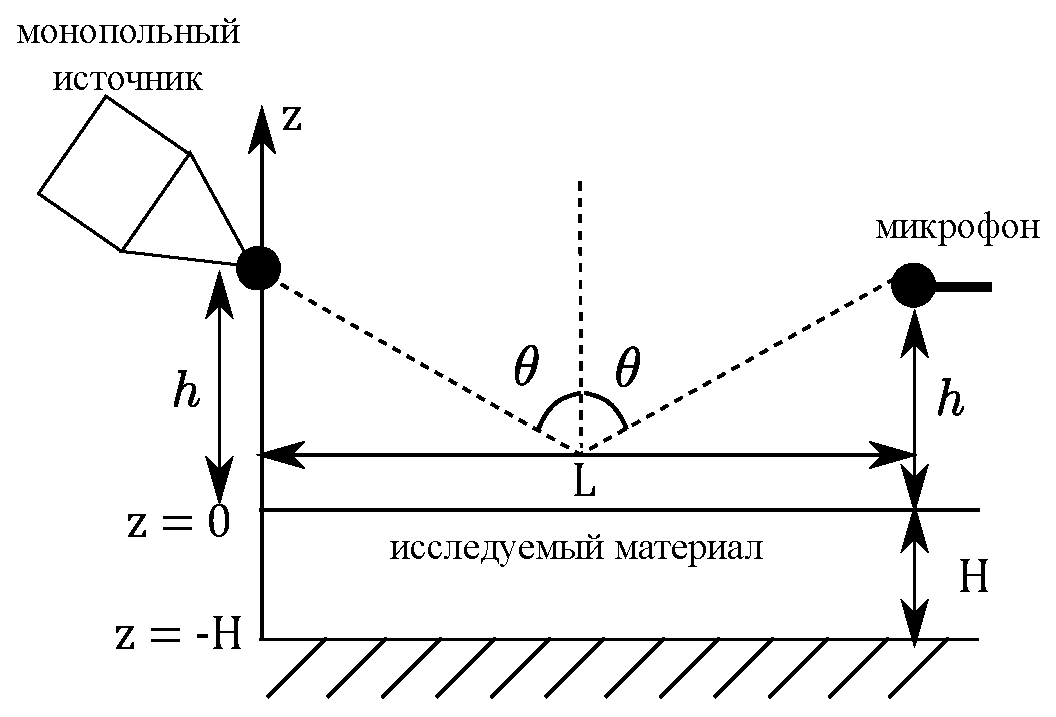
\includegraphics [scale=0.8] {ris1_1}
	\caption{Схема эксперимента.}
	\label{img:ris1_1}
\end{figure}

Акустические волны в среде возбуждает монопольный источник, находящийся в точке $(0, 0, h), h > 0$. Приемник расположен в точке  $(L, 0, h)$.
 
Поле точечного источника опишем неоднородным волновым уравнением
\begin{equation}
\label{eq:waveequation}
\frac{1}{c_0^2} \frac{\partial^2 p}{\partial t^2} - \Delta p = \rho_0 \frac{\partial W(t)}{\partial t} \delta(x) \delta(y) \delta(z-h),
\end{equation}
где $W(t)$ – объем воздуха, производимого в единицу времени источником, измеряется в $\text{м}^3$/\text{с}; $c$ - скорость звука в воздухе.

В эксперименте измеряется набор импульсных откликов для углов падения $\theta_n$. Из каждого импульсного отклика при помощи преобразования Фурье вычисляется частотная характеристика $P_n(\omega)$ отраженного от образца поля для каждого угла падения $\theta_n$. При обработке из частотных характеристик получается частотная зависимость коэффициента отражения от образца при данном угле падения.

\section{Описание поля сферической волны. Интеграл Фурье-Бесселя}

Рассмотрим стационарную задачу распространения гармонической волны с частотой $f$. В этом случае $W(t) = Be^{-i\omega t}$, $\omega = 2\pi f$. Экспоненциальная зависимость всех величин от времени будет далее опущена. Решение стационарной задачи будет представлять собой сумму прямого и отраженного поля:

\begin{equation}
P = P_d + P_r.
\end{equation}

Прямое поле $P_d$ на приемнике вычисляется по формуле монопольного источника \cite{Isakovich1973}:

\begin{equation}
\label{eq:pointsource}
P_d(\omega, r) = - \frac{i\omega\rho_0 \exp{i k_0 L}}{4 \pi r} w(\omega),
\end{equation}
где $w(\omega)$ - Фурье-образ $W(t)$, $k_0 = \omega / c_0$, $\omega = 2 \pi f$.

Отраженное поле дается интегралом Фурье-Бесселя \cite{Biot1956_I, Biot1956_II}:

\begin{multline}
\label{eq:reflectedfield}
P_r(\omega, 2h, L) = w(\omega) \frac{\omega \rho_0}{4 \pi} \int_{0}^{\infty} \frac{k_{||} R(\omega, \arcsin(k_{||}/k_0) ) J_0(k_{||}L)}{\sqrt{k_0^2 - k_{||}^2}} \\
 \exp(i \sqrt{k_0^2 - k_{||}^2} 2h) dk_{||},
\end{multline}  
где $k_{||} = k_0 \sin\varphi$ – величина проекции волнового вектора на плоскость $Oxy$, $\varphi = \arcsin\left(\frac{k_{||}}{k_0}\right)$, $R$ – коэффициент отражения плоской волны, падающей под углом к нормали $\varphi = \arcsin(k_{||}/k_0)$. Коэффициент отражения определяется свойствами материала и его толщиной. В настоящей работе исследуется вспененный меламин, который описывается моделью Био для пористых сред \cite{Biot1956_I, Biot1956_II}. Для материалов, которые описываются этой моделью, было получено аналитическое выражение для коэффициента отражения в \cite{Allard2009}.

В эксперименте непосредственно измеряется полное поле $P = P_r + P_d$ для разных положений источника и приемника. Затем путем обработки из него выделяется величина $P_r$, из нее строится оценка для коэффициента отражения. Простейшая оценка коэффициента отражения может быть получена путем деления $P_r$ на поле монопольного источника ~\eqref{eq:pointsource}. Такая оценка, очевидно, будет справедлива только в том случае, когда источник находится достаточно далеко от поверхности исследуемого материала. Действительно, в этом случае поле излучаемое источником близко к полю плоской волны, которое отражается с коэффициентом, близким к $R$. Оценим с помощью формулы ~\eqref{eq:reflectedfield} точность такой оценки для случая нормального падения. Учитывая, что $J_0(0) = 1$, и оценивая оставшийся интеграл с помощью метода перевала, получим:
  		
\begin{multline}
\label{eq:reflectedfield2}
P_r(\omega, 2h, 0) = R(\omega, 0) P_d(\omega, 2h) + P_d(\omega, 2h) R'(\omega, 0) \sqrt{\frac{\pi i}{2k_0(2h)}} +  \\
O([k_0(2h)]^{-2}),
\end{multline}
где штрих обозначает частную  производную по второму аргументу. В эксперименте $2h \sim 1$  м, следовательно, оценка коэффициента отражения по первому члену в ~\eqref{eq:reflectedfield2} будет справедлива на частотах выше 500 Гц. Кроме того, второй член в ~\eqref{eq:reflectedfield2} позволяет апостериорно оценить корректность аппроксимации путем вычисления производной $R'$.



\section{Отыскание коэффициента отражения с помощью обращения интеграла Фурье-Бесселя}

Более точная оценка для коэффициента отражения может быть построена с помощью приближенного обращения интеграла Фурье-Бесселя. Переходя от переменной $k_{||}$ к переменной $\varphi = \arcsin\left(\frac{k_{||}}{k_0}\right)$ в ~\eqref{eq:reflectedfield}, получим:

\begin{equation}
\label{eq:fb_change_vars}
\tilde{P}_r(\omega, \theta, h) = w(\omega) \frac{\omega \rho_0}{4 \pi} \int_{\Gamma} k_0 \sin \varphi R(\omega, \varphi) J_0\left(\frac{2 k_0 h \sin \varphi}{\tan \theta}\right) e^{2 i k_0 h \cos \varphi} d \varphi,
\end{equation}
где $\tilde{P}_r(\omega, \theta, h) = P_r(\omega, 2h, \frac{2h}{\tan \theta})$, а контур $\Gamma$ изображен на (Рис. \ref{img:ris1_2}). Пусть из эксперимента известен набор функций $P_n = \tilde{P}_r(\omega, \theta_n, h)$ при заданных $\theta_n$, $1\leq n \leq N$. В интеграле ~\eqref{eq:fb_change_vars} заменим $R(\varphi)$ на некоторую интерполяцию 
\begin{equation}
\label{eq:reflectionsum}
\tilde{R}(\omega, \varphi) = \sum_{m=1}^{N} R_m(\omega) E_m(\varphi),
\end{equation}
где $E_m$ – интерполяционные функции, а $R_m(\omega)$ – функции, подлежащие определению. Подставляя ~\eqref{eq:reflectionsum} в ~\eqref{eq:fb_change_vars} и проводя интегрирование, получим следующее матричное уравнение: 
\begin{equation}
\label{eq:mainequation}
P_n = M_{nm}R_m,
\end{equation}
где
\begin{equation}
\label{eq:Mnm}
M_{nm} = w(\omega) \frac{\omega \rho_0}{4 \pi} \int_{\Gamma} k_0 \sin\varphi E_m(\varphi) J_0\left(\frac{2k_0 h \sin\varphi}{\tan\theta_n}\right) e^{2ik_0 h \cos \varphi} d\varphi.
\end{equation}

\begin{figure}[ht]
	\centering
	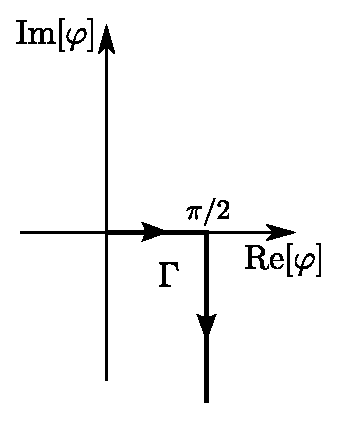
\includegraphics [scale=1] {ris1_2}
	\caption{Контур интегрирования.}
	\label{img:ris1_2}
\end{figure}

Решая уравнение ~\eqref{eq:mainequation}, определим неизвестные коэффициенты $R_m$ и, пользуясь формулой ~\eqref{eq:reflectionsum}, получим оценку для коэффициента отражения. Корректность построенной оценки сильно зависит от выбранных интерполяционных функций. Если на заданном наборе $\theta_n$ коэффициент отражения меняется плавно, то на участке $[0; \pi/2]$ функции $E_n$ могут быть выбраны кусочно-линейными:

\begin{equation}
\label{eq:shapefunctions}
E_n(\varphi)=
\begin{cases}
0, \varphi \leq \theta_{n-1}, \varphi \geq \theta_{n+1} \\
\dfrac{\theta_{n+1} - \varphi}{\theta_{n+1} - \theta_n}, \theta_n < \varphi < \theta_{n+1} \\
\dfrac{\varphi - \theta_n}{\theta_{n+1} - \theta_n}, \theta_{n-1} < \varphi < \theta_n
\end{cases}
\end{equation}

Отметим, что если $E_n$ выбраны в соответствии с ~\eqref{eq:shapefunctions}, то коэффициенты $R_m(\omega)$ являются приближением к коэффициенту отражения $R(\omega, \theta_m)$ .

Остановимся на деталях численной реализации. 

Важной задачей является выбор последней функции $E_n(\varphi)$ при мнимых $\varphi$. В данной работе $E_n(\varphi) = 1, \text{Im}[\varphi] < 0$ . Данный выбор был обусловлен следующими соображениями. При $h \neq 0$ такой выбор слабо влияет на результат ввиду экспоненциального затухания подынтегрального выражения в ~\eqref{eq:Mnm}. Однако при $h = 0$, когда быстрого затухания нет, получается постоянный коэффициент отражения при мнимых углах, что соответствует модели Био (при касательном падении меламин ведет себя как граница Дирихле).

Хорошо известно, что задача решения уравнения 

\begin{equation}
R_m = M_{nm}^{-1} P_n
\end{equation}
является некорректно поставленной, так как матрица $M_{nm}$ плохо обусловлена, и непосредственное ее численное обращение может вести к значительным численным ошибкам. Поэтому при решении уравнения ~\eqref{eq:mainequation} применялась регуляризация Тихонова

\begin{equation}
R_m = (M_{nm}^T M_{nm} + \lambda I)^{-1} M_{nm}^{-1} P_n,
\end{equation}
где $I$ - единичная матрица, а параметр $\lambda$ выбирался исходя из численных экспериментов. На частотах от $500$ до $2000$ Гц выбиралось значение $\lambda = 0.2$, на более высоких частотах регуляризация не требовалась.

\section{Описание эксперимента}

Геометрия эксперимента соответствует Рис. ~\ref{img:ris1_1}. Параметры $h$ и $L$ подбирались таким образом, чтобы расстояние, проходимое отраженным сигналом, было порядка 1 метра.

\begin{figure}[ht]
	\centering
	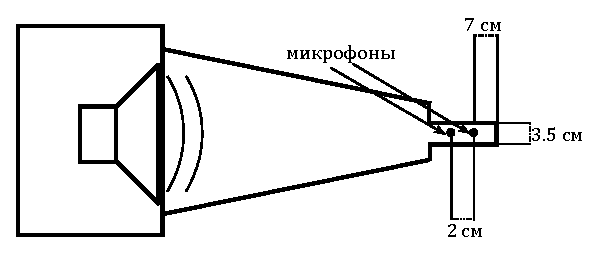
\includegraphics [scale=1] {ris1_3}
	\caption{Схема монопольного источника.}
	\label{img:ris1_3}
\end{figure}

В качестве монопольного источника использовался аналог Bruel \& Kjaer 4295 Omnisource, выполненный из фанерного короба с клиновидным концентратором (Рис. \ref{img:ris1_3}). К источнику крепится адаптер для измерения объемной скорости. Адаптер представляет собой отрезок металлической трубы диаметром $3,5$ см с двумя отверстиями для микрофонов, расстояние между которыми $2$ см. Это расстояние определяет наивысшую частоту, для которой возможно определение колебательной скорости ($8,5$ кГц). Это ограничение следует из метода двух микрофонов \cite{ASTM}. Для регистрации поля и измерения объемной скорости использовались $6$ мм микрофоны Audix TM1, обладающие достаточно ровной частотной характеристикой в широком диапазоне частот. 
	
Импульсный отклик определялся с помощью метода \textit{M}-последовательности. Подробно данная техника описана в \cite{ValyaevMLS}. Остановимся здесь лишь на основных моментах. \textit{M}-последовательность – это двухуровневый квазишумовой сигнал с количеством отсчетов $2^M - 1$, где для данной работы $M = 19$ (длительность около $11$ секунд с частотой дискретизации $48$ кГц). \textit{М}-последовательность подается на ЦАП и воспроизводится источником. Затем принимаются сигнал с микрофона, расположенного в точке приема и пара сигналов  с двух микрофонов, помещенных в адаптер объемной скорости. Вычисляется кросс-корреляция каждого из сигналов с исходной \textit{M}-последовательностью. На корреляционные функции накладывается временное окно, чтобы выделить первые несколько метров принятого сигнала и отрезать весь остальной сигнал. Затем с каждым из сигналов производится преобразование Фурье. Из сигналов, полученных с микрофонов в адаптере, вычисляется Фурье-спектр объемной скорости при помощи формулы двух микрофонов с учетом поправки Вайнштейна, описывающей отражение от открытого конца волновода \cite{Weinstein1966}. Отношение спектра давления в точке приема к спектру объемной скорости источника дает частотный отклик всего акустического тракта. 
	
Далее выполняется фильтрация фильтром низких частот с частотой отсечки $4500$ Гц и шириной $500$ Гц. Фильтрация позволяет избежать импульсов с большими пиковыми величинами. Для удобства результат нормируется таким образом, чтобы амплитуда пика от прямого сигнала была единичной при расстоянии от источника до микрофона $1$ м. После фильтрации к полученному сигналу применяется обратное преобразование Фурье. Обратное преобразование Фурье дает профильтрованный импульсный отклик. 

Поскольку эксперимент имел хорошую повторяемость, была возможность улучшить соотношение сигнал/шум, вычитая из отклика, полученного при наличии отражения от исследуемого материала, отклик свободного поля без материала. Сначала проводился эксперимент с отражением от исследуемого материала Рис. ~\ref{img:ris1_4}, линия из точек. Затем исследуемый материал и жесткая подложка убирались, и импульсный отклик измерялся снова. Так получался отклик свободного поля, который вычитался из отклика, полученного с отражением от материала, и так повышалось отношение амплитуд сигнала и шума в отклике Рис. ~\ref{img:ris1_4}, сплошная линия. Из полученного таким образом импульсного отклика при помощи гладкой маски (Рис. ~\ref{img:ris1_4}, пунктирная линия) вырезается часть, соответствующая отраженному сигналу. Фурье-образ вырезанной части представляет собой отраженное поле $P_r$.

\begin{figure}[ht]
	\centering
	\label{img:ris1_4}
	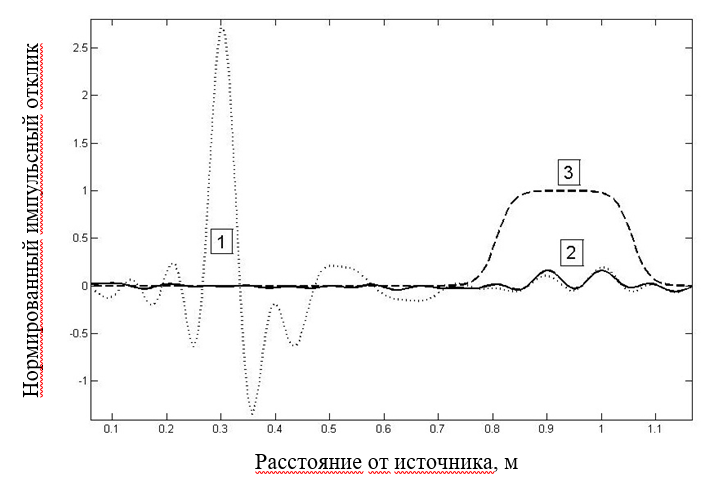
\includegraphics [scale=0.75] {ris1_4}
	\caption{Пример импульсного отклика. По горизонтальной оси отложено расстояние от источника, по вертикальной оси отложена амплитуда импульсного отлика. Линия из точек соответствует сигналу до вычитания отклика свободного поля; сплошная линия – сигналу после вычитания; пунктирная линия – маске, необходимой для выделения участка, соответствующего отражению от меламина. Пик 1 соответствует прямому сигналу от источника; пара пиков 2 соответствует сигналу, отраженному от меламина (один пик от поверхности меламина, другой от подложки, на которую он наклеен); маска 3 предназначена для выделения отраженного сигнала.}
\end{figure}

Проводится серия таких экспериментов для разных углов падения $\theta$. С помощью методов, описанных в предыдущем разделе, строится оценка для коэффициента отражения.

\section{Экспериментальные результаты}

Для проверки работоспособности предлагаемой методики и построенной экспериментальной установки были проведены эксперименты по измерению импульсного отклика исследуемого материала с углами $\theta = 0 ^{\circ}, 15 ^{\circ}, 30 ^{\circ}, 45 ^{\circ}, 60 ^{\circ}$ (см. Рис. ~\ref{img:ris1_1}). Из модели Био известно, что с изменением угла $\theta$ величина коэффициента отражения меняется плавно, поэтому такого небольшого набора углов должно быть достаточно. К сожалению, измерения для больших углов $\varphi$ были затруднены ввиду наложения прямого и отраженного сигнала в импульсном отклике. К тому же, имелись проблемы, связанные с конечным размером образца: на низких частотах образец оказывается меньше размера первой зоны Френеля, и тогда, если расстояние от источника до образца около $0,5$ м, сторона образца должна быть около $1,5$ м. 
	
После окончания измерений получается набор частотных характеристик $P_n = \tilde{P}_r(\omega, \theta_n, h)$ для каждого угла падения $\theta_n$. После того, как по формулам ~\eqref{eq:reflectedfield2} и ~\eqref{eq:reflectionsum}, ~\eqref{eq:mainequation} были получены оценки для коэффициента отражения, они сравнивались с такой же зависимостью, вычисленной по модели Био с учетом толщины образца при помощи переходной матрицы. Метод вычисления теоретической зависимости описан в \cite{Allard2009}.

\begin{figure}[ht]
	\centering
	\label{img:ris1_5}	
	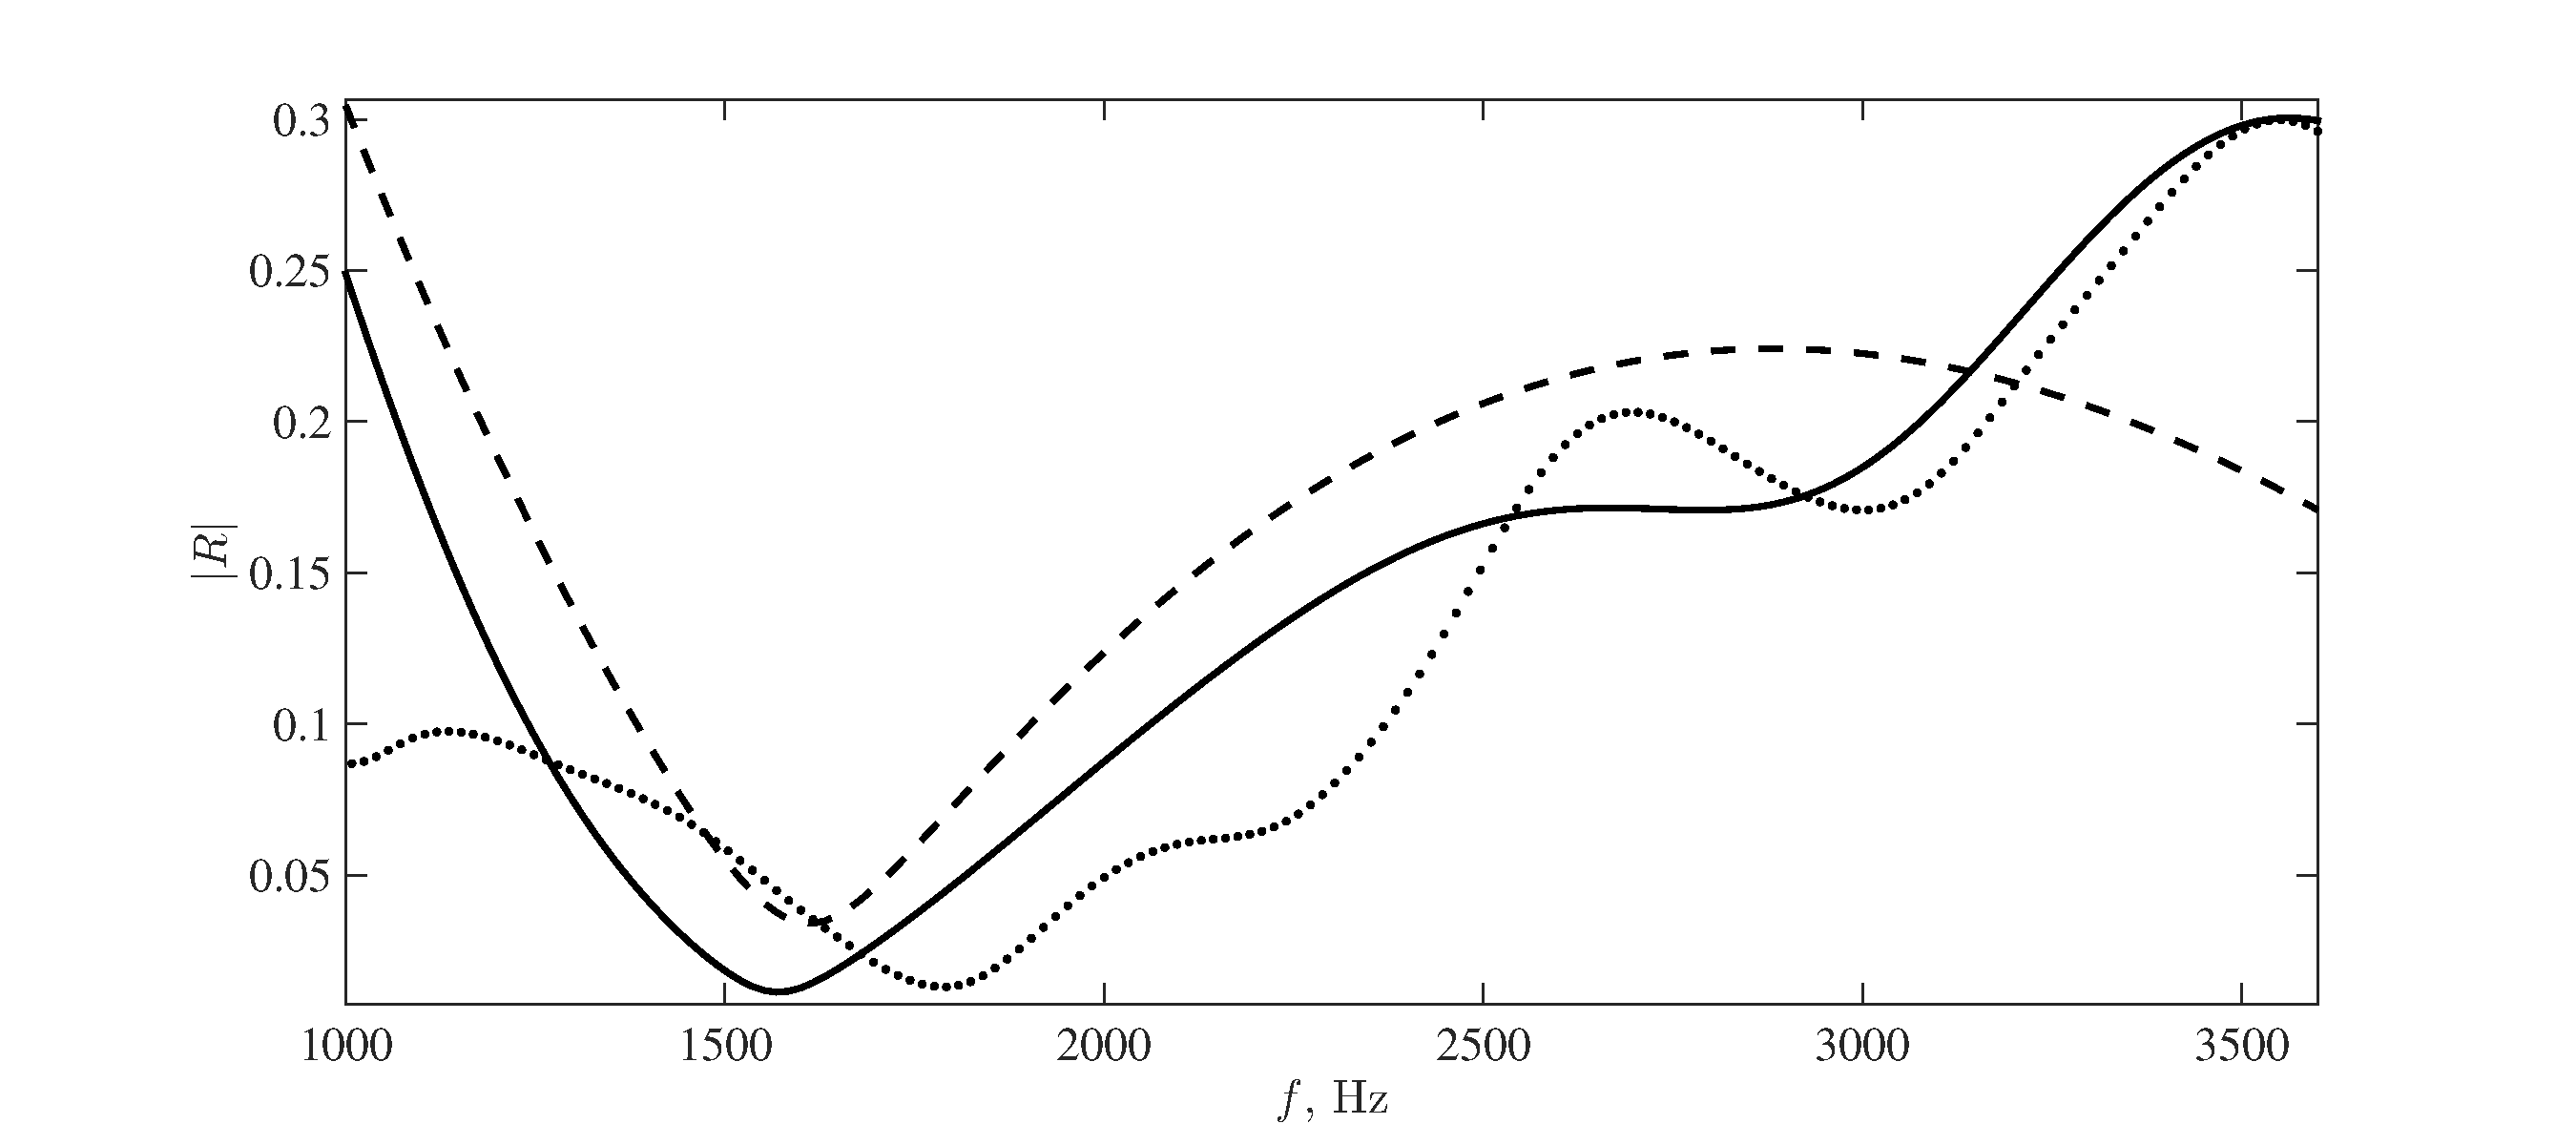
\includegraphics [scale=0.4] {ris1_5}
	\caption{График зависимости модуля коэффициента отражения $|R|$ при угле падения равном $0^\circ$. Пунктирной линией обозначен результат, полученный с помощью формулы ~\eqref{eq:reflectedfield2}, точками – с помощью формул ~\eqref{eq:reflectionsum}, ~\eqref{eq:mainequation}, сплошной линией – результат теоретического расчета на основе модели Био.}
\end{figure}

\begin{figure}[ht]
	\centering
	\label{img:ris1_6}	
	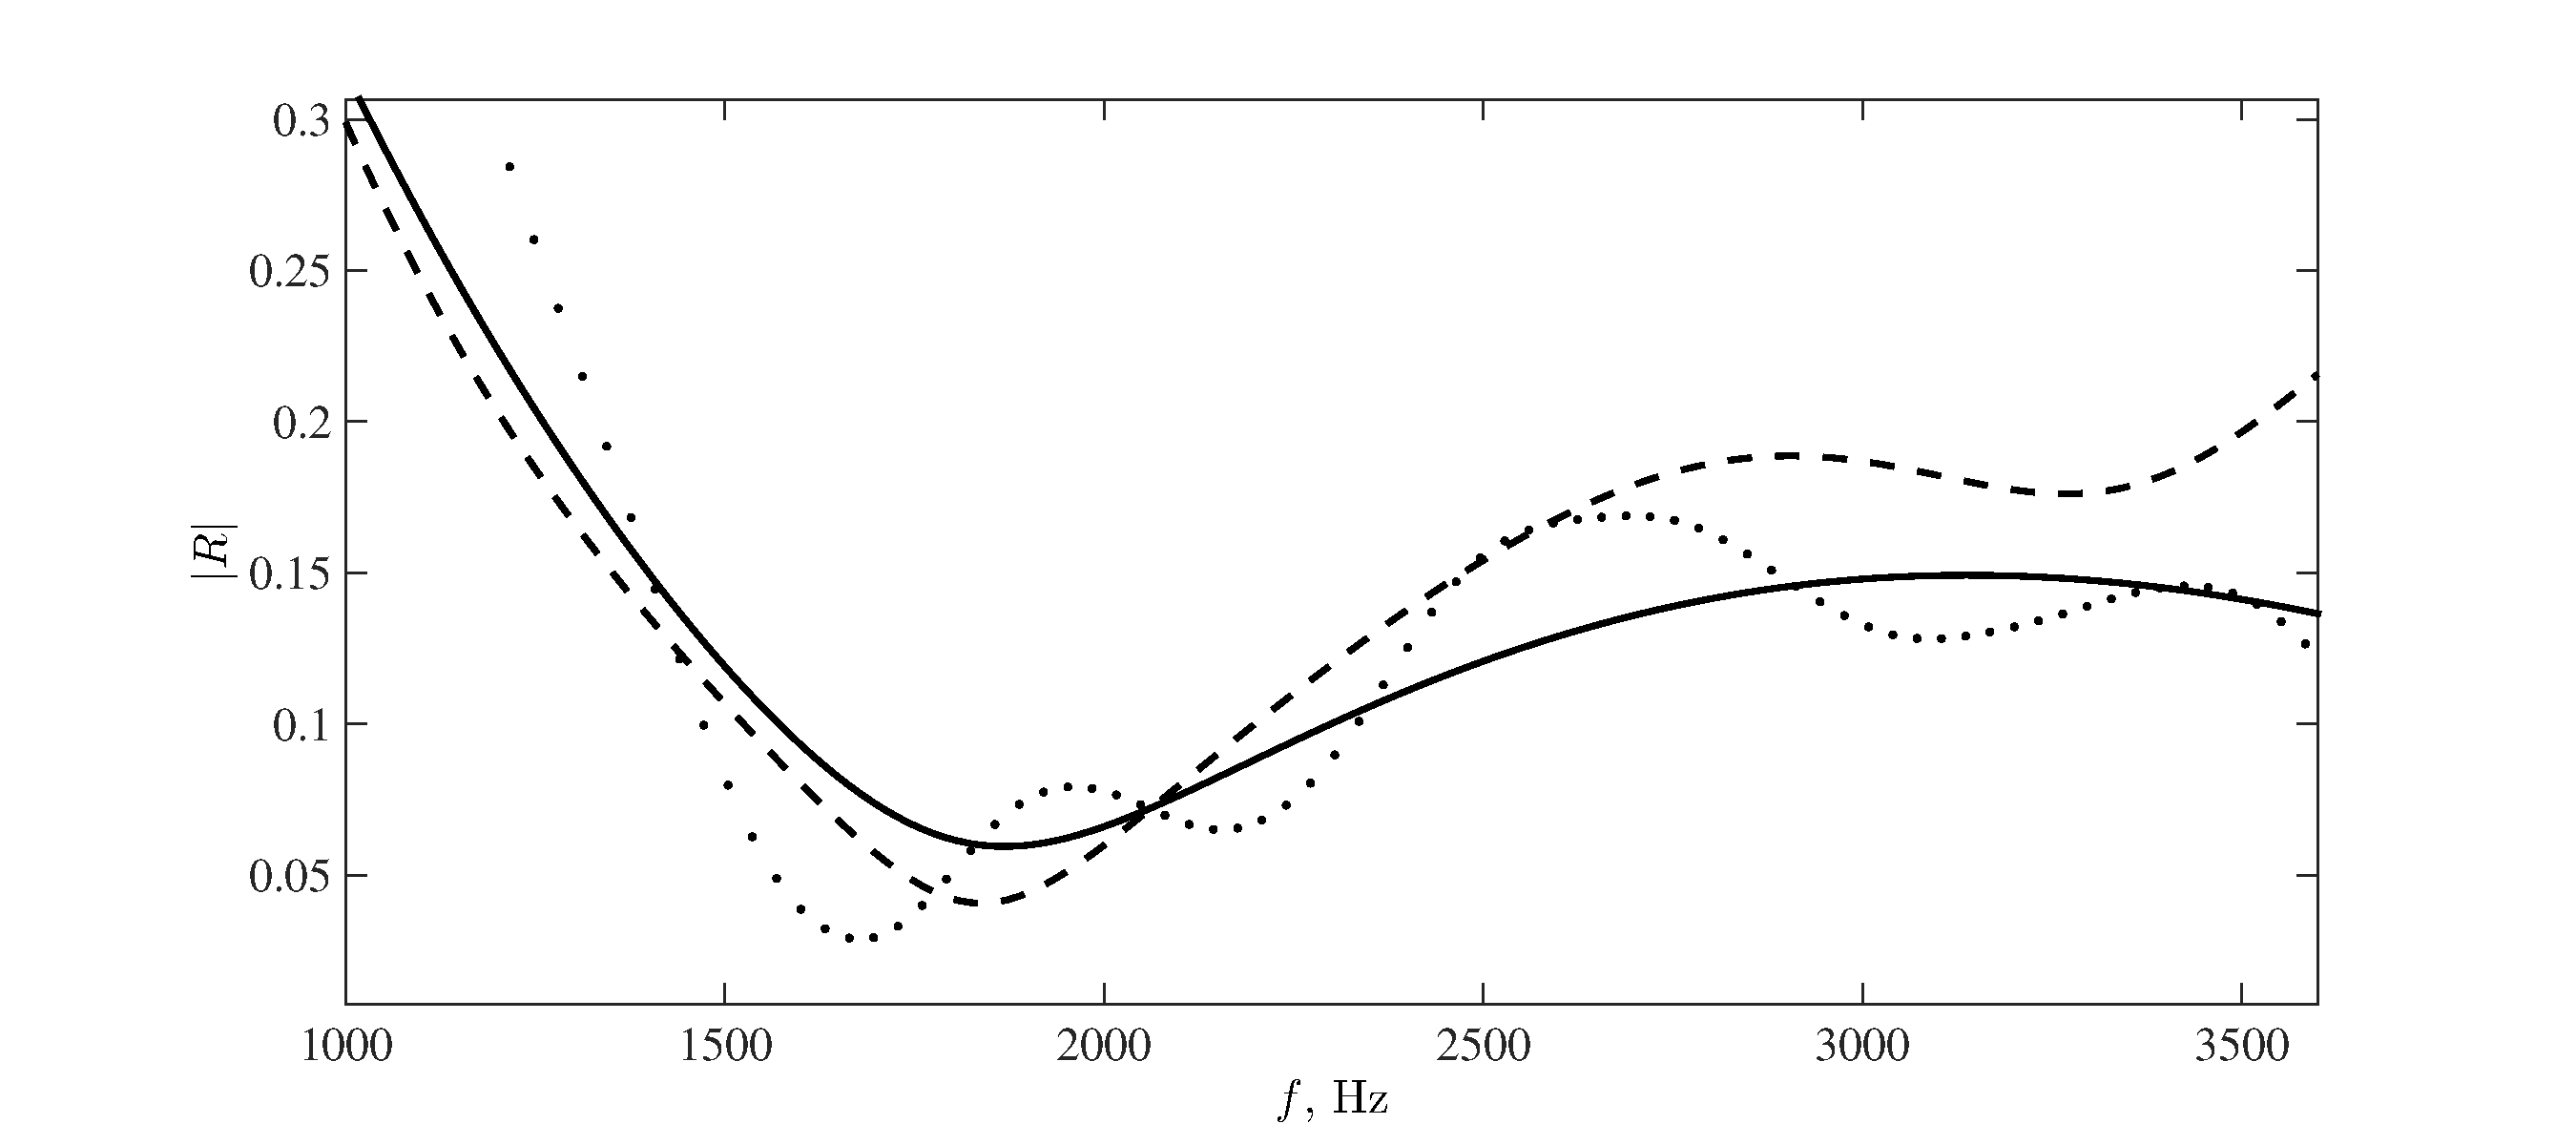
\includegraphics [scale=0.4] {ris1_6}
	\caption{График зависимости модуля коэффициента отражения $|R|$ при угле падения равном $30^\circ$. Пунктирной линией обозначен результат, полученный с помощью формулы ~\eqref{eq:reflectedfield2}, точками – с помощью формул ~\eqref{eq:reflectionsum}, ~\eqref{eq:mainequation}, сплошной линией – результат теоретического расчета на основе модели Био.}
\end{figure}

\begin{figure}[ht]
	\centering
	\label{img:ris1_7}
	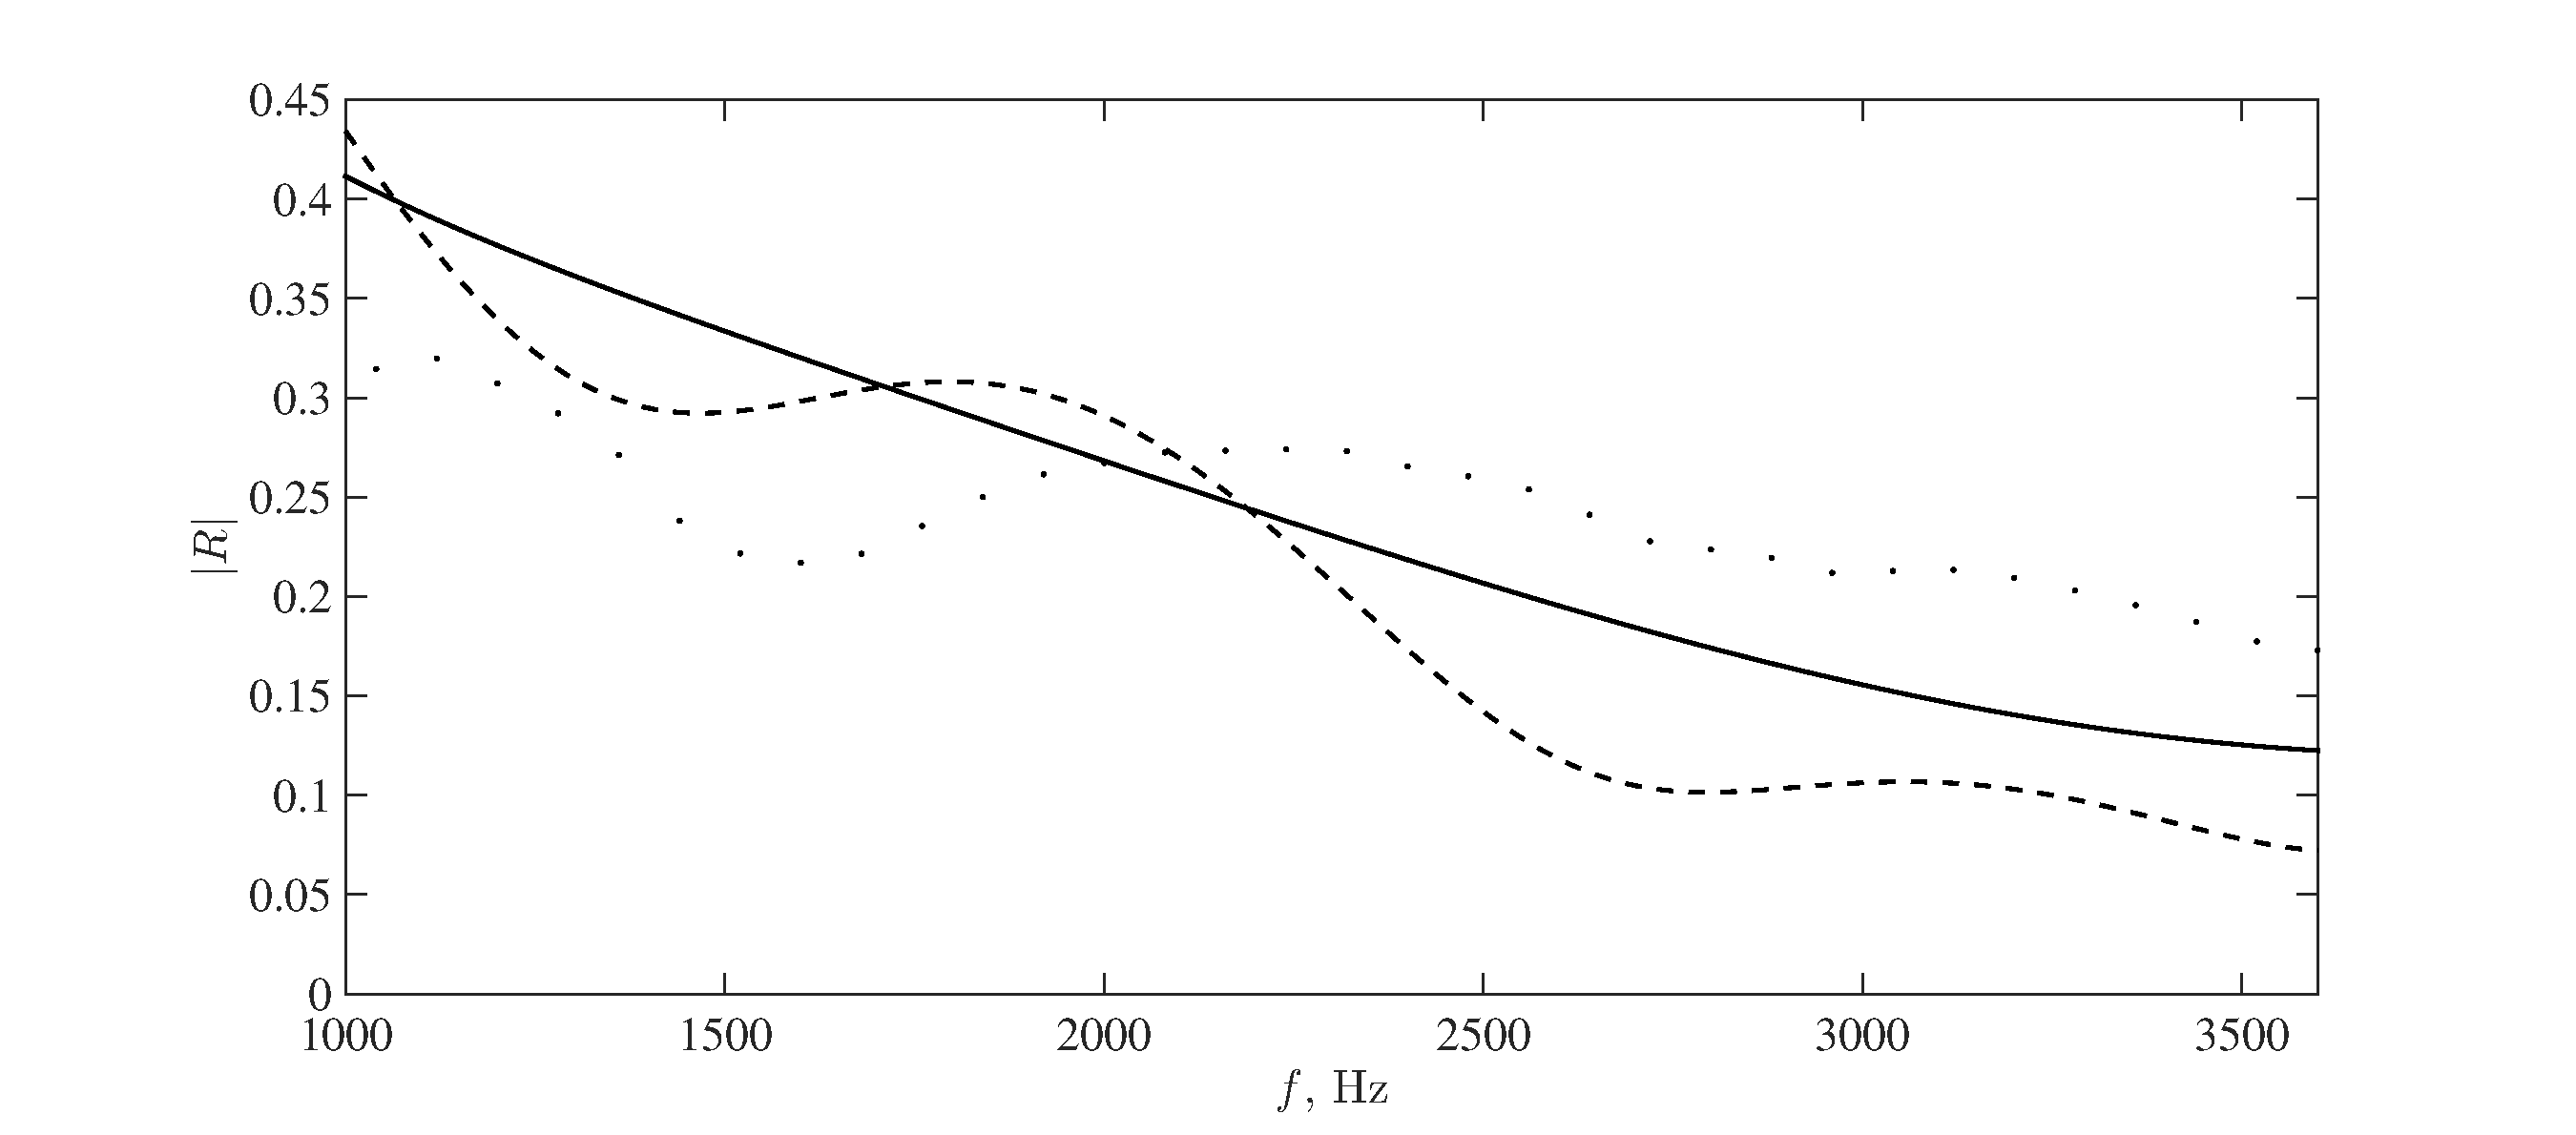
\includegraphics [scale=0.4] {ris1_7}
	\caption{График зависимости модуля коэффициента отражения $|R|$ при угле падения равном $60^\circ$. Пунктирной линией обозначен результат, полученный с помощью формулы ~\eqref{eq:reflectedfield2}, точками – с помощью формул ~\eqref{eq:reflectionsum}, ~\eqref{eq:mainequation}, сплошной линией – результат теоретического расчета на основе модели Био.}
\end{figure}

Результаты сравнения действительных частей коэффициентов отражения для нескольких частот представлены на Рис. ~\eqref{img:ris1_5}, ~\eqref{img:ris1_6}, ~\eqref{img:ris1_7}. Пунктирной линией обозначен результат, полученный с помощью формулы ~\eqref{eq:reflectedfield2}, точками – с помощью формул ~\eqref{eq:reflectionsum}, с кусочно-линейными интерполяционными функциями ~\eqref{eq:shapefunctions}, сплошной линией – результат теоретического расчета на основе модели Био \cite{Biot1956_I, Biot1956_II}. В качестве параметров модели Био использовались параметры, измеренные экспериментально в работе \cite{Geebelen2007} (см. таблицу).

\begin{table}
	\label{tabular:melamine}
	\begin{center}
		\begin{tabular}{cc}
			Пористость (\textit{англ.} porosity) [1] $\Phi$ & $0.99$ \\
			Сопротивление потоку (\textit{англ.} flow resistivity) $\sigma$ $[\text{Нм}^{-4} с]$ & $12000$ \\
			Термическая проницаемость (\textit{англ.} thermal permeability) $k'_0$ $[1]$ & $1.5 \times 10^{-9}$\\
			Масштаб вязкости (\textit{англ.} viscous dimension) $\Lambda$ $[\text{м}]$ & $100\times 10^{-6}$ \\	
			Тепловой масштаб (\textit{англ.} thermal dimension) $\Lambda'$ $[\text{м}]$ & $400\times 10^{-6}$\\
			Плотность материала $\rho_s$ $[\text{кг/м}^3]$ & $9$\\
			Сдвиговый модуль $N$ $[\text{кПа}]$ & $86(1 + 0.05i)$\\
			Коэффициент Пуассона $\nu$ & $0.276$
		\end{tabular}
	\end{center}
	\caption{Параметры пористого меламина.}
\end{table}

Как видно из Рис. ~\eqref{img:ris1_5}, ~\eqref{img:ris1_6}, ~\eqref{img:ris1_7}, при углах падения, для которых проводился эксперимент, описанная техника дает удовлетворительное соответствие с теорией Био и может быть использована для измерения угловых зависимостей коэффициентов отражения для имеющихся и новых звукопоглощающих материалов. Некоторое несоответствие экспериментальных и теоретических результатов авторы объясняют внутренними шумами экспериментальной установки, ошибками в измерении геометрии эксперимента и тем, что образец исследуемого материала был собран из различных прямоугольных кусков, слегка отличающихся по форме и свойствам.
